\subsection{Progettazione di dettaglio e codifica}

\subsubsection{Prospetto orario}
Nel periodo di progettazione di dettaglio e codifica la distribuzione oraria è la seguente:

\renewcommand{\arraystretch}{1.5}
\begin{table}[H]
\begin{center}
\begin{tabular}{|c|c|c|c|c|c|c|c|}
\hline
\rowcolor{title_row}
\textbf{\color{title_text}{Nome}} & \textbf{\color{title_text}{Resp.}} & \textbf{\color{title_text}{Ammi.}} & \textbf{\color{title_text}{Analist.}} & \textbf{\color{title_text}{Progett.}} & \textbf{\color{title_text}{Program.}} & \textbf{\color{title_text}{Verific.}} & \textbf{\color{title_text}{Totale}} \\ \hline
Andrea Trevisin  & & 8 & & 10 & 19 & 16 & 53  \\ \hline
Giacomo Barzon   & 4 & 5 & & 11 & 19 & 16 & 55 \\ \hline
Giovanni Sorice  & 6 & & & 12 & 20 & 14 & 52  \\ \hline
Lorenzo Busin    & 7 & 3 & & 13 & 19 & 13 & 55  \\ \hline
Marco Costantino & & & 5 & 14 & 20 & 15 & 54 \\ \hline
Michele Roverato & & 4 & & 11 & 22 & 15 & 52  \\ \hline
Nicolò Tartaggia & & & 5 & 10 & 21 & 17 & 53  \\ \hline
\end{tabular}
\caption{Tabella 5.4.1: Distribuzione oraria del periodo "Progettazione di dettaglio e codifica"\label{}}
\end{center}
\end{table}
\renewcommand{\arraystretch}{1}

Il seguente grafico dà una rappresentazione visiva della suddivisione oraria: \\
\begin{figure} [H]
	\centering
	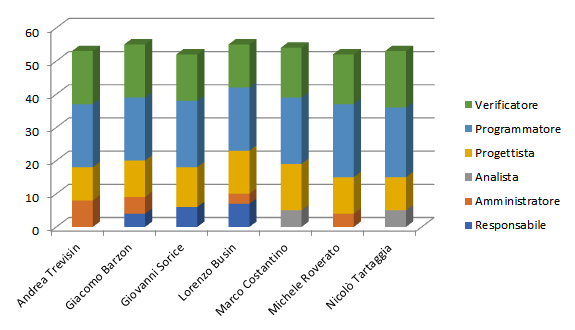
\includegraphics[scale=1]{Res/ExcelGrafici/Grafici/CodificaOre.png}
	\caption{Figura 5.4.1: Grafico suddivisione oraria del periodo "Progettazione di dettaglio e codifica"}\label{}
\end{figure}


\subsubsection{Prospetto economico}
Nel periodo di progettazione di dettaglio e codifica il resoconto della distribuzione delle ore e dei relativi costi è la seguente:

\renewcommand{\arraystretch}{1.5}
\begin{table}[H]
\begin{center}
\begin{tabular}{|c|c|c|}
\hline
\rowcolor{title_row}
\textbf{\color{title_text}{Ruolo}}  & \textbf{\color{title_text}{Ore}} & \textbf{\color{title_text}{Costo in \euro}} \\ \hline
Responsabile    & 17           & 510                 \\ \hline
Amministratore  & 20           & 400                 \\ \hline
Analista        & 10           & 250  	               \\ \hline
Progettista     & 81           & 1.782                \\ \hline
Programmatore   & 140          & 2.100                \\ \hline
Verificatore    & 106          & 1.590                \\ \hline
\textbf{Totale} & \textbf{374}    & \textbf{6.632}           \\ \hline
\end{tabular}
\caption{Tabella 5.4.2: Prospetto economico del periodo "Progettazione di dettaglio e codifica"\label{}}
\end{center}
\end{table}
\renewcommand{\arraystretch}{1}

Il seguente grafico dà una rappresentazione visiva della distribuzione dei ruoli: \\
\begin{figure} [H]
	\centering
	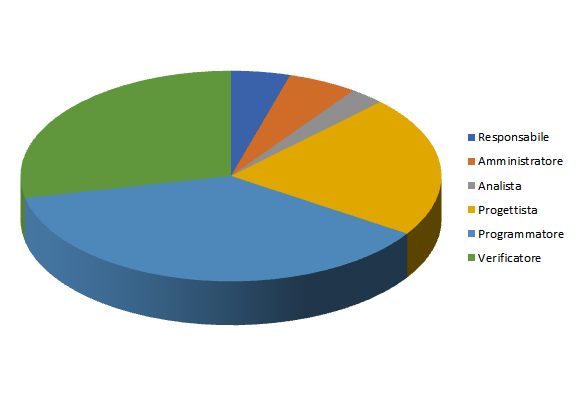
\includegraphics[scale=1]{Res/ExcelGrafici/Grafici/CodificaRuoli.png}
	\caption{Figura 5.4.2: Grafico suddivisione dei ruoli del periodo "Progettazione di dettaglio e codifica"}\label{}
\end{figure}

\pagebreak
